% 薄透镜

% 球形界面
% 未完成: 改名为透镜

\pentry{折射定律\upref{Snel}}

\begin{figure}[ht]
\centering
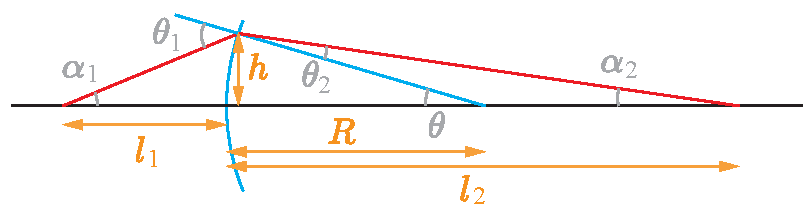
\includegraphics[width=12.5cm]{./figures/ThnLen1.pdf}
\caption{单球面成像}} \label{ThnLen_fig1}
\end{figure}

如\autoref{ThnLen_fig1}, 我们考虑两种折射率分别为 $n_1$ 和 $n_2$ 得介质被一个球面划分为左右两部分. 当光线从左边入射时, 经过界面反射.

\textbf{傍轴条件}: 图中所有角度都很小\footnote{即 $\sin\beta \approx \tan\beta \approx \beta$, 见 “小角正弦极限\upref{LimArc}”}. 球面近似是平面, 球面上任意一点横坐标相同.
\begin{equation}
l_1 \alpha_1 = l_2 \alpha_2 = R\theta
\end{equation}
由三角形性质得
\begin{equation}
\alpha_1 = \theta_1 - \theta \qquad
\alpha_2 = \theta - \theta_2
\end{equation}

\begin{equation}
n_1 \theta_1 = n_2 \theta_2
\end{equation}
消去 $\theta_1$ 和 $\theta_2$ 得
\begin{equation}
\frac{n_1}{l_1} + \frac{n_2}{l_2} = \frac{n_2 - n_1}{R}
\end{equation}
这已经比较接近凸透镜成像公式了. 注意 $l_1, l_2$ 取负数时同样成立.

对于薄透镜, 就得到了成像公式
\begin{equation}
\frac{1}{u} + \frac{1}{v} = \frac{1}{f}
\end{equation}
其中
\begin{equation}
\frac{1}{f} = \qty(\frac{n_2}{n_1} - 1) \qty(\frac{1}{R_1} + \frac{1}{R_2})
\end{equation}
